\section{Motivation and Background}
\label{background}

Single GPU performance has been scaling very well amassing a significant
growth in per-GPU transistor count and DRAM BW. For example a 2010 Nvidia's
529mm\textsuperscript{2} Fermi GPUs integrated 1.95B transistors with 180 GB/s
DRAM bandwidth, while 2016 Nvidia 610 mm\textsuperscript{2} Pascal GPUs reached
a 12B transistor count with 720 GB/s memory bandwidth. Unfortunately transistor density
growth slows down and expected to come to a halt at 7nm. Moreover, as GPU die sizes
have been also increasing over the past generations, this growth is expected to
slow down due to limitations in lithography and manufacturing costs. 
Without larger or denser dies, GPU manufacturers are likely to turn to 
alternative technologies such as the tried and trued solution from CPU world,
the \textit{multi-socket GPUs}, to keep scaling effective GPU perfromance via 
growing overall transistor counts and DRAM bandwidths. 

%One moving to 3D die-stacking as a solution for continued transistor growth. 
%Unfortunately 3D die-stacking still has a significant number of engineering 
%challenges related to power delivery, energy density, and 
%cooling~\cite{verbree2010cost} when employed in maximal die-sized chips such as 
%GPUs and moving beyond a 2 high stack to 4 or 8 stacks will be even more 
%difficult. Because of these challenges, 
%GPU manufacturers are likely to 
%consider a tried and trued solution in the CPU world to gain additional 
%transistor count, \textit{multi-socket GPUs}.

\begin{figure*}[tp] 
    \centering
    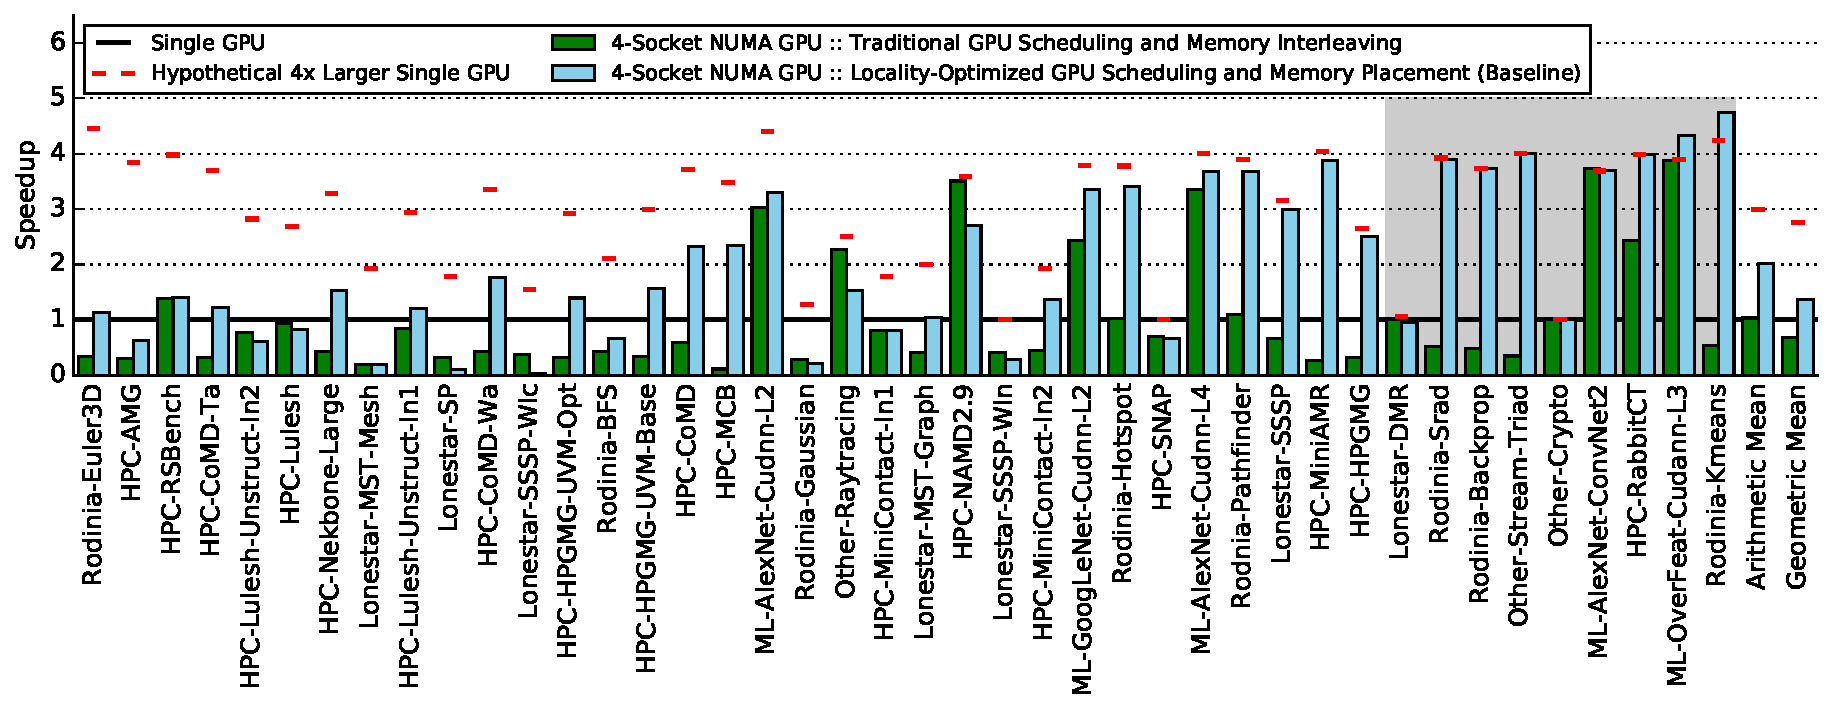
\includegraphics[width=1.0\linewidth]{figures/plot_different_baselines.pdf}
    \caption{Relative performance of a 4-socket NUMA GPU using to a single GPU 
and a hypothetical 4$\times$ larger (all resources scaled) single GPU showing 
upper bound of performance this application can achieve via GPU hardware 
scaling. For the Locality-Optimized design, applications shown in grey 
achieve already 99\% of theoretical scaling (\emph{red dash}) without 
microarchitectural modification.}
    \label{fig:motivation}
\end{figure*}

The evolution of GPU computing has moved from it being a PCIe attached peripherals 
to computing platforms designed around the GPU as the primary computing engine. 
Such systems epmloy custom PCB designs that accommodate multiple high pin count socketed 
GPUs~\cite{DGX} with inter-GPU interconnects resembling QPI or 
Hypertransport~\cite{INTELQPI,AMDHT} much more than legacy PCIe interfaces.  
Despite the improvement in hardware capabilities, to-date these multi-GPU 
solutions have been exposed as a collection of single GPU solutions with improved GPU--GPU 
interconnects. While multi-GPU systems can provide high aggregate throughput, 
the programming models for multi-GPU systems has diverged from the single GPU 
programming model and requires layering additional software runtimes like MPI 
or openshmem on top of the native GPU programming interfaces such as CUDA or openCL.
By requiring re-writing of the GPU application to enable multi-GPU performance, 
many applications are never ported to use multiple GPUs.

In this work, we examine the performance achievable by architecting a 
multi-socket NUMA-aware single GPU.  Building upon existing work in the 
NUMA-CPU and GPU community, we first describe the basic multi-socket GPU runtime 
that allows a multi-socket GPU system to be exposed to GPU developers as a 
single GPU and exploits some well known scheduling and memory locality 
optimizations for NUMA systems. We then look at the performance implications 
that this multi-socket NUMA design has on applications that have been optimized 
for a traditional single GPU.  We identify that current GPU interconnect 
utilization and cache policies are sub-optimal for a multi-socket NUMA GPU and 
show how these problems can largely be overcome with architectural innovation.  
Finally, we examine the scaling efficiency of a multi-socket NUMA-aware GPU to 
understand if NUMA-aware GPUs will see significantly improve performance  
without any code-rewriting required by the application programmer.

